\documentclass{article}
\usepackage[margin=1in]{geometry}
\usepackage{problemset}
\showsolntrue

% Custom commands
\newcommand{\R}{\mathbb{R}}
\newcommand{\X}{\mathcal{X}}
\newcommand{\Y}{\mathcal{Y}}
\newcommand{\E}{\mathbb{E}}
\newcommand{\V}{\text{Var}}
\renewcommand{\P}{\mathbb{P}}

\begin{document}

\pstitle{%
    MATH 189%
}{
    Homework 6%
}[due Tuesday, March 4 at 8:00AM]

\textbf{Resources:} These problems appear in Ch. 10 of the textbook pgs. 465-467.

\textbf{Format requirements:} Type your homeworks using \LaTeX with embedded plots for the applied exercises.

\textbf{Grading:} The grading is based 50\% on completion and 50\% on correctness.

\vspace{1em}

\begin{probset}

% --- Problem 1 ---
\begin{prob}[\textbf{Ch. 10 conceptual exercise 1}]
    Consider a neural network with two hidden layers: $p = 4$ input units, $2$ units in the first hidden layer, $3$ units in the second hidden layer, and a single output.

    \begin{subprobset}
        \begin{subprob}
            Draw a picture of the network, similar to Figures 10.1 or 10.4 in the textbook.

            \begin{soln}
                \begin{center}
                    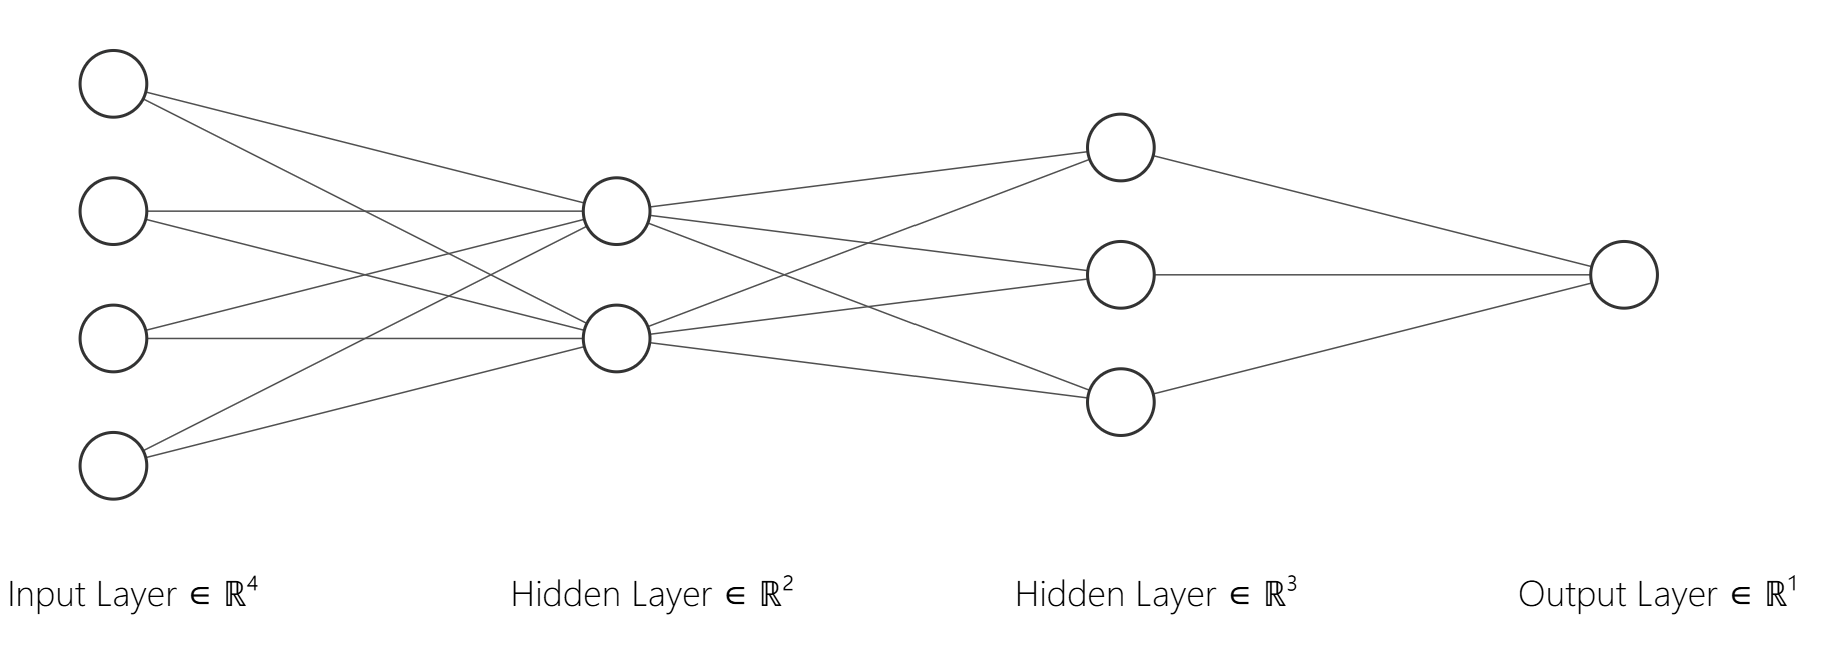
\includegraphics[width=0.8\textwidth]{Images/1a.png}
                \end{center}
            \end{soln}
        \end{subprob}

        \begin{subprob}
            Write out an expression for $f(x)$, assuming ReLU activation functions. Be as explicit as you can!

            \begin{soln}
                \begin{align*}
                    f(x) &= \max(0, w^T\max(0, W_2 \max(0, W_1 x + b_1) + b_2) + b_3)
                \end{align*}
            \end{soln}
        \end{subprob}

        \begin{subprob}
            Now plug in some values for the coefficients and write out the value of $f(x)$.

            \begin{soln}
                Let $x = \begin{bmatrix} 1 & 1 & 0 & 0 \end{bmatrix}^T$, $W_1 = \begin{bmatrix} 1 & 1 & 0 & 0 \\ 0 & 0 & 1 & 1 \end{bmatrix}$, $b_1 = \begin{bmatrix} 0 \\ 0 \end{bmatrix}$, $W_2 = \begin{bmatrix} 1 & 0 \\ 1 & 1 \\ 0 & 1 \end{bmatrix}$, $b_2 = \begin{bmatrix} -1 \\ 0 \\ -1 \end{bmatrix}$, $w = \begin{bmatrix} 1 & 1 & 1 \end{bmatrix}^T$, $b_3 = 0$.

                $h_1 = \max(0, W_1 x + b_1) = \begin{bmatrix} 2 & 0 \end{bmatrix}^T$, $h_2 = \max(0, W_2 h_1 + b_2) = \begin{bmatrix} 1 & 2 & 0 \end{bmatrix}^T$
                
                $f(x) = \max(0, w^T h_2 + b_3) = \boxed{3}$
            \end{soln}
        \end{subprob}

        \begin{subprob}
            How many parameters are there?

            \begin{soln}
                \[
                    (4 + 1) \times 2 + (2 + 1) \times 3 + (3 + 1) \times 1 = 10 + 9 + 4 = 23
                \]
            \end{soln}
        \end{subprob}
    \end{subprobset}
\end{prob}

\newpage

% --- Problem 2 ---
\begin{prob}[\textbf{Ch. 10 conceptual exercise 4}]
    Consider a CNN that takes in $32 \times 32$ grayscale images and has a single convolution layer with three $5 \times 5$ convolution filters (without boundary padding).

    \begin{subprobset}
        \begin{subprob}
            Draw a sketch of the input and first hidden layer similar to Figure 10.8 in the textbook.

            \begin{soln}
                \begin{center}
                    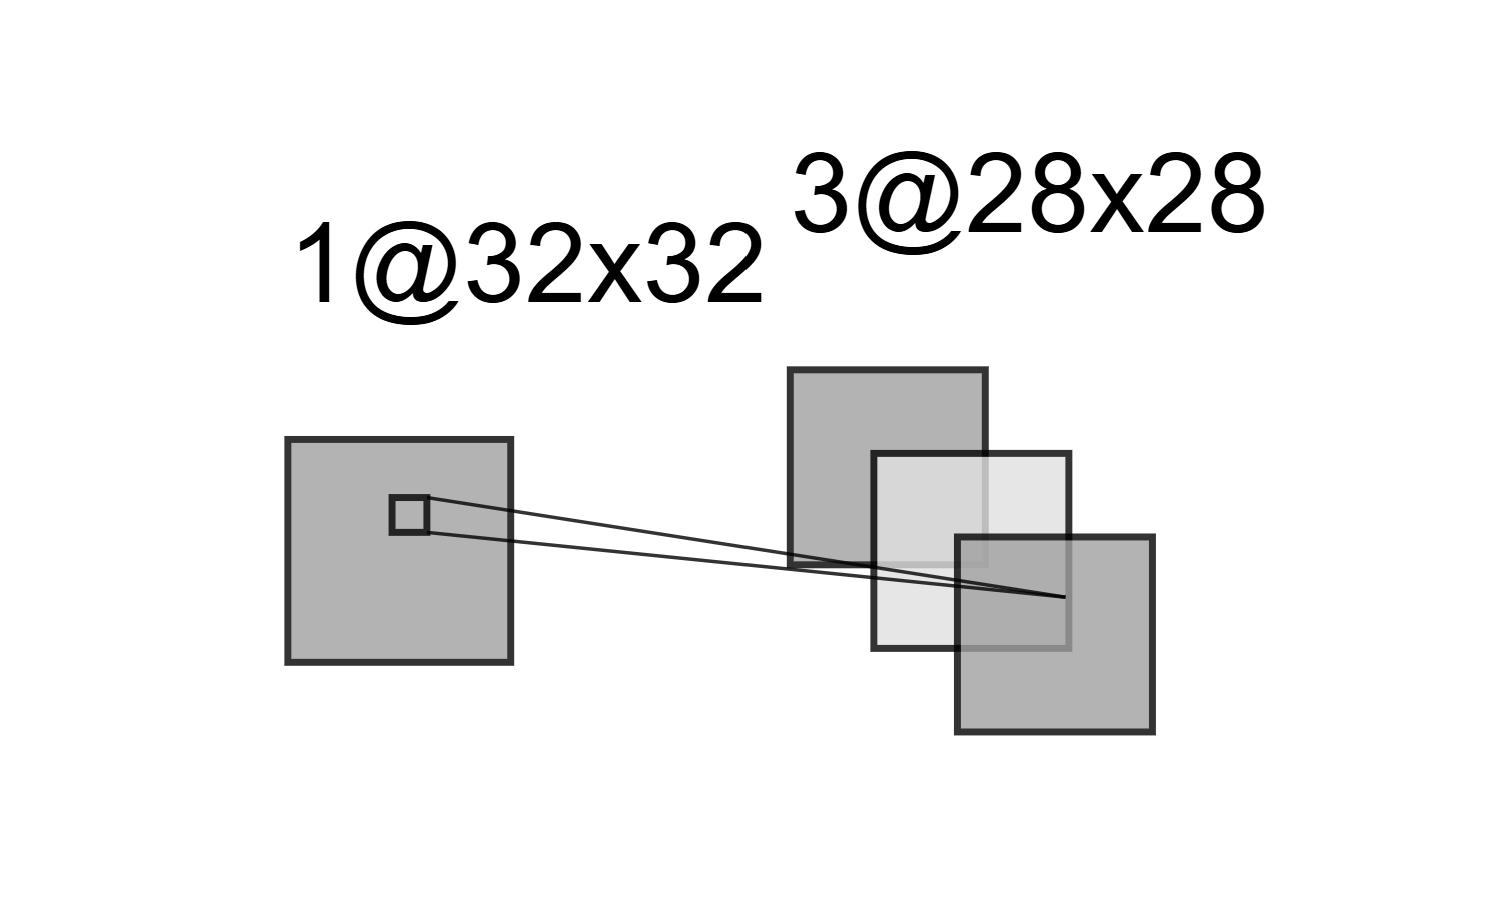
\includegraphics[width=0.5\textwidth]{Images/2a.png}
                \end{center}
            \end{soln}
        \end{subprob}

        \begin{subprob}
            How many parameters are in this model?

            \begin{soln}
                \[
                    3 \times (5 \times 5 + 1) = 3 \times 26 = 78
                \]
            \end{soln}
        \end{subprob}

        \begin{subprob}
            Explain how this model can be thought of as an ordinary feedforward neural network with the individual pixels as inputs, and with constraints on the weights in the hidden units. What are the constraints?

            \begin{soln}
                In the feedforward view, inputs are the 1024 pixels. Hidden units are the $3 \times 28 \times 28 = 2352$ outputs (one per filter position). Each hidden unit takes a $5 \times 5$ patch of the input (25 pixels).

                The constraints are the same 25 weights are used at every spatial position for a given filter. That is, the filter weights are shared across all positions where the filter is applied.
            \end{soln}
        \end{subprob}

        \begin{subprob}
            If there were no constraints, then how many weights would there be in the ordinary feed-forward neural network in (c)?

            \begin{soln}
                Without sharing weights, there would be $3 \times 28 \times 28 \times (5 \times 5 + 1) = 61,152$ weights.
            \end{soln}
        \end{subprob}
    \end{subprobset}
\end{prob}

\newpage

% --- Problem 3 ---
\begin{prob}[\textbf{Ch. 10 applied exercise 6}]
    Consider the simple function $R(\beta) = \sin(\beta) + \beta/10$.

    \begin{subprobset}
        \begin{subprob}
            Draw a graph of this function over the range $\beta \in [-6, 6]$.

            \begin{soln}
                \begin{center}
                    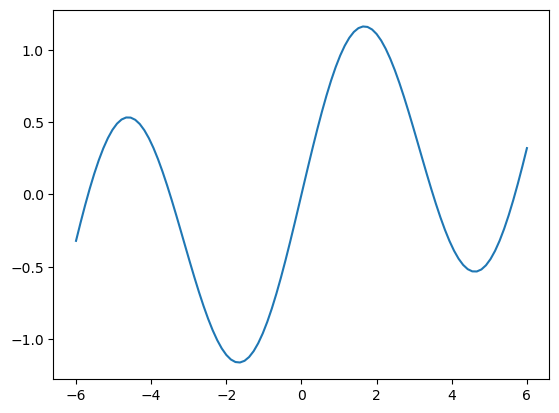
\includegraphics[width=0.38\textwidth]{Images/3a.png}
                \end{center}
            \end{soln}
        \end{subprob}

        \begin{subprob}
            What is the derivative of this function?

            \begin{soln}
                $R'(\beta) = \cos(\beta) + 1/10$
            \end{soln}
        \end{subprob}

        \begin{subprob}
            Given $\beta_0 = 2.3$, run gradient descent to find a local minimum of $R(\beta)$ using a learning rate of $\rho = 0.1$. Show each of $\beta_0, \beta_1, \ldots$ in your plot, as well as the final answer.

            \begin{soln}
                \begin{center}
                    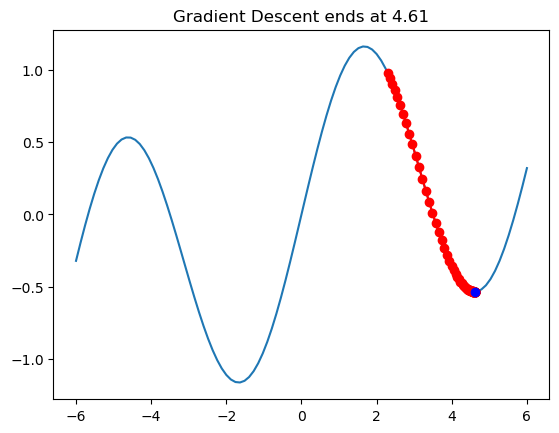
\includegraphics[width=0.38\textwidth]{Images/3c.png}
                \end{center}
            \end{soln}
        \end{subprob}

        \begin{subprob}
            Repeat with $\beta_0 = 1.4$.

            \begin{soln}
                \begin{center}
                    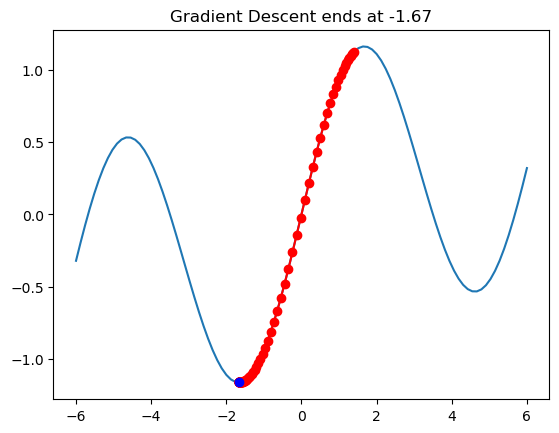
\includegraphics[width=0.38\textwidth]{Images/3d.png}
                \end{center}
            \end{soln}
        \end{subprob}
    \end{subprobset}
\end{prob}

\newpage

% --- Problem 4 ---
\begin{prob}[\textbf{Ch. 10 applied exercise 7 with different regularization}]
    Fit a neural network to the \texttt{Default} data. Use a single hidden layer with 10 units and any time of regularization (the book uses dropout regularization, weight decay is more modern). Have a look at Labs 10.9.1-10.9.2 for guidance. Compare the classification performance of your model with that of linear logistic regression.

    \begin{soln}
        \begin{center}
            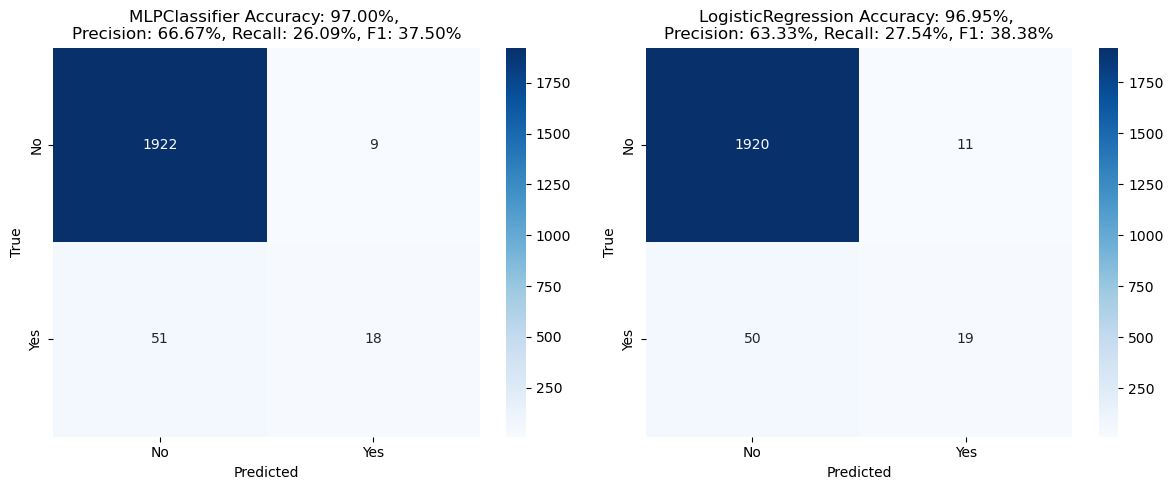
\includegraphics[width=0.8\textwidth]{Images/4.png}
        \end{center}
        Both models had similarly high accuracy scores and similarly low F1 scores. This is because most of the labels were 0, so the data is imbalanced. With balanced data, the accuracies are slightly lower, but the F1 scores are much higher. Here, they are also almost exactly the same.
        \begin{center}
            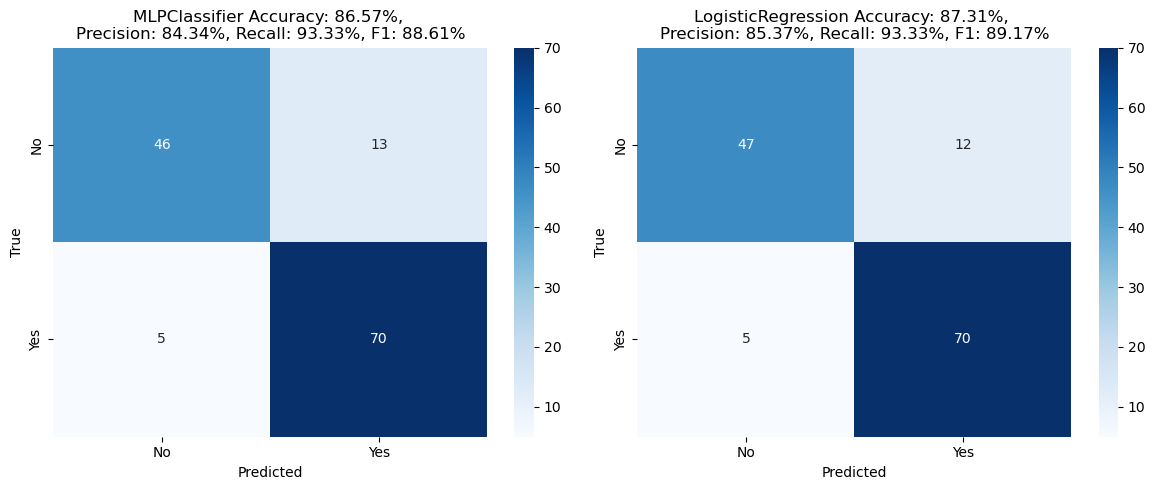
\includegraphics[width=0.8\textwidth]{Images/4b.png}
        \end{center}
    \end{soln}
\end{prob}
\end{probset}
\end{document}